\documentclass[conference]{IEEEtran}
\IEEEoverridecommandlockouts
% The preceding line is only needed to identify funding in the first footnote. If that is unneeded, please comment it out.
\usepackage{cite}
\usepackage{url}
\usepackage{hyperref}
\usepackage{amsmath,amssymb,amsfonts}
\usepackage{algorithm}
\usepackage{algorithmic}
\usepackage{graphicx}
\usepackage{subcaption} 
\usepackage{textcomp}
\usepackage{xcolor}
\def\BibTeX{{\rm B\kern-.05em{\sc i\kern-.025em b}\kern-.08em
    T\kern-.1667em\lower.7ex\hbox{E}\kern-.125emX}}
\newcommand{\fk}[1]{\textcolor{red}{[FK:#1]}}
\begin{document}

\title{\textbf{Learning and generalizing manipulation tasks on humanoid robots with automatic, multisensory segmentation methods}
}

\author{\IEEEauthorblockN{Victor Barberteguy$^{1,2}$}
\IEEEauthorblockA{}
\and
\IEEEauthorblockN{Fumio Kanehiro$^{2}$}
\IEEEauthorblockA{}
\thanks{$^{1}$Ecole Polytechnique, Palaiseau, France}
\thanks{$^{2}$CNRS-AIST JRL (Joint Robotics Laboratory), IRL, National Institute of Advanced Industrial Science and Technology (AIST), Japan}
}

\maketitle

\begin{abstract}
We provide a complete framework for learning and reproducing tasks from human demonstrations. This method adapts recent developments in automatic, unsupervised segmentation of time-series to humanoid robotics by preprocessing the data obtained from a broad range of the robot's sensors, to then repropduce and generalize the learned task in similar environments.

In more detail,  we reproduce and extend the acquired multi-step task using Dynamic Movement Primitives in simulation for the JVRC1 Robot, and further validate it in the real world with the HRP-4C Robot, thus showcasing the capacity of our approach to create an extensive library of reusable skills for complex humanoids.
\end{abstract}

\begin{IEEEkeywords}
learning from demonstration, generalization, teleoperation, probabilistic inference, feature selection, dynamic movement primitives, sensory skill integration
\end{IEEEkeywords}

\fk{try to shorten (especially Section II) to six pages for the initial submission. For example, as we are just using DMP, II-B can be completely removed.}
\section{Introduction}
\subsection{Learning from Demonstration}

Demonstrations provide an intuitive way for non-professional users to specify tasks to the robot \cite{schaal_is_1999}. Most of robot's controllers to date, albeit successful to achieve complex tasks, often require theoretical knowledge and is time-consuming. To address these issues, research about robot learning from demonstration (LfD) has become increasingly important over the past two decades with the surge of Machine Learning (ML) algorithms \cite{argall_survey_2009} \cite{ravichandar_recent_2020}. In this framework, users can demonstrate a task that is then learned and generalized by the robot. Generalization is defined as the capacity to perform a learned task in a similar environment as the one of the demonstration, but under different initial or goal poses. LfD has been widely used and proved successful on robotic arms or in simulation \cite{pastor_learning_2009}, but are more seldom used on real humanoid robots \cite{calinon_learning_2007} due to their high number of degrees of freedom (DoF) and unlinear behavior. A core idea of this work is to capitalize on the physiologic similarities between us, humans, and humanoids robots to come up with an intuitive LfD technique. Consequently, this article showcases a method specific to humanoid robots.


\begin{figure}[t]
  \centering
  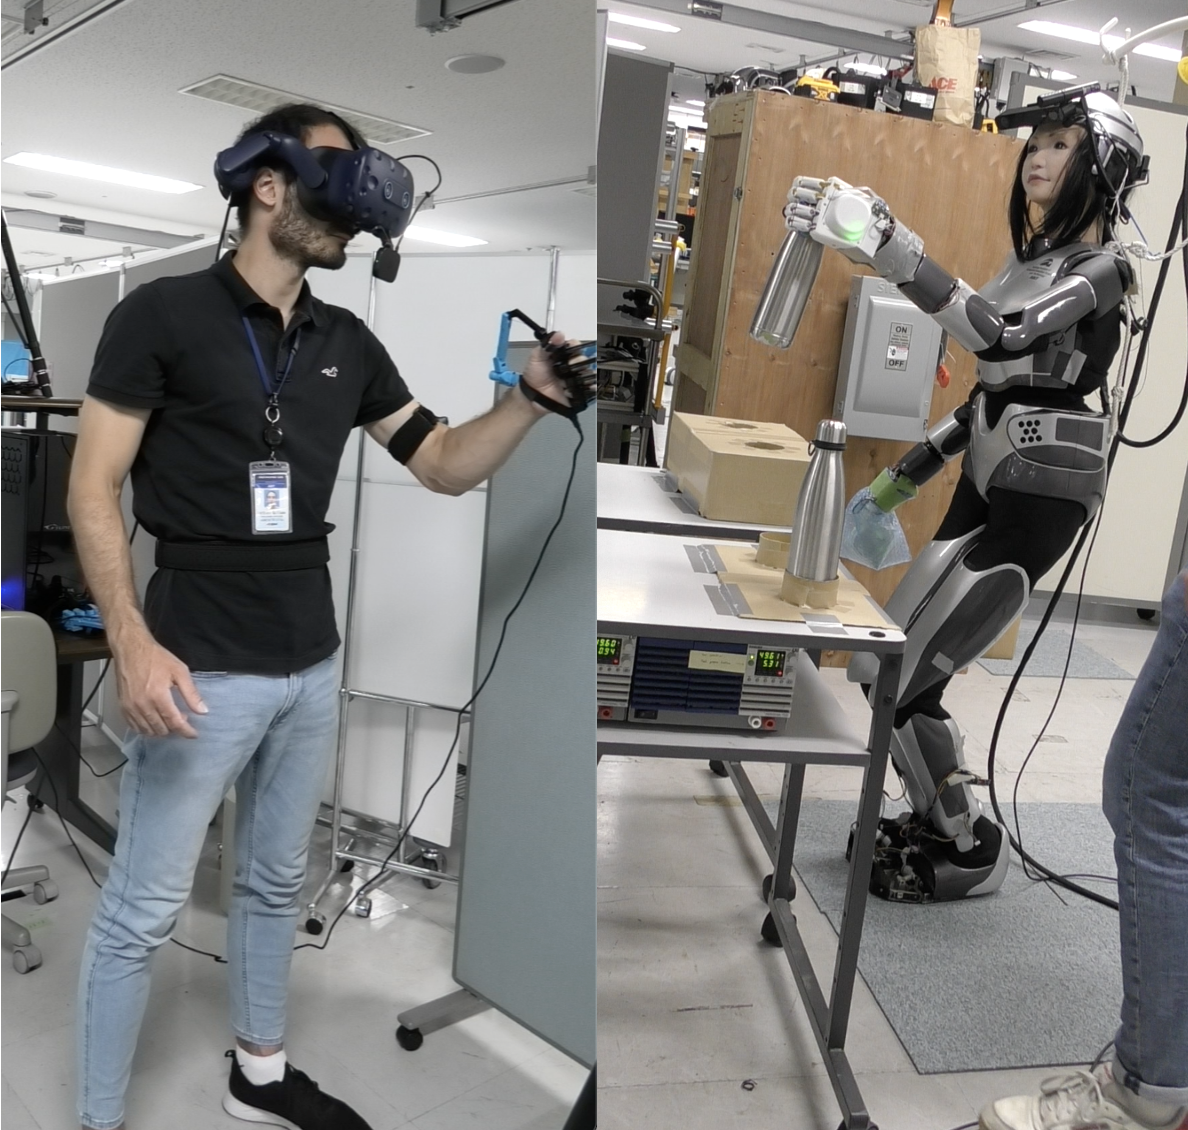
\includegraphics[width=0.45\textwidth]{img/Setup.png}
  \caption{Picture of the experimental setup. On the right, the demonstrator wearing the teleoperation device. On the left, the HRP-4C robot that is teleoperated}
  \label{fig:setup}
\end{figure}


Several techniques are found in the literature to provide demonstrations to the robot. This can be done through simulation \cite{sammut_learning_1992}, kinesthesic teaching \cite{wu_prim-lafd:_2022}, motion capture \cite{ramirez-amaro_understanding_2015} or with teleoperation devices. These teleoperations devices appear under various shapes, from joysticks \cite{ando_master-slave_2020} to exoskeletons where the user remotely controls the robot \cite{fang_skill_2019}. In all the above cited works, some prefer 1-shot imitation learning, where the demonstration can be a seed for an initial policy that is then derived and learned through Reinforcement Learning (RL) \cite{vecerik_practical_2019} \cite{stulp_reinforcement_2012}, Inverse RL \cite{rouot_inverse_2017} or Hierarchical RL \cite{zhao_variational_2023} that can possibly be corrected with online coaching \cite{advice_operator}. Another recent approach is to create more demonstrations with the initial one, thus enriching the dataset thanks to meta-learning processes \cite{yu_one-shot_2018}. On the contrary, other methods rely on a set of demonstrations to perform probabilistic inference based on Hidden Markov Models \cite{rana_towards_2017}, Neural Networks \cite{zhang_deep_2018} or using Granger Causality \cite{chuck2023grangercausal}. The former often derives only one policy that is locally optima, and thus the learning process is repeated for each task, whereas the latter methods prefer to decompose the task in elementary \textit{skills} with segmentation methods, thus enhancing the reusability of the stored skills. Our proposed method is of the latter category, that is further detailed in \ref{Approach}

Whatever the method used, once the task learned, the great majority of the references cited above use Dynamic Movement Primitives (DMP), that were first introduced by Ijspeert and Schaal in \cite{ijspeert_movement_2002} and futher explored in \cite{ijspeert_dynamical_2013}. It provides a suitable framework to reproduce trajectories and to smoothly adapt to new conditions.

\subsection{Related work} \label{Approach}

Splitting a complex task such as grasping an object or pouring water has the advantage of making the result more generalizable. Indeed, every part of the trajectory (every \textit{skill}) has its own level of generalizability thanks to DMP, thus resulting in an intra-task generalization, better than a single end-to-end DMP. Nonetheless, a complex task is almost all the time demonstrated without specifying the number of segments: the demonstrator naturally achieves the task. Consequently, one challenge of this approach is to automatically segment the trajectory in human-interpretable skills that, once stored in a library, can be reused to learn new skills \cite{meier_movement_2011}.

Recent methods provide plans to the robot about the different phases of the demonstration using natural language or computer vision \cite{caccavale_kinesthetic_2019} \cite{saran_enhancing_2019}. Besides, probabilistic approaches are employed to segment a demonstration in a unsupervised fashion. The number of phases involved as well as the temporal position of changepoint (CP) are inferred automatically. These techniques include Hidden Markov Models (HMM) \cite{niekum_learning_2015}, Gaussian Mixture Regression (GMR) \cite{calinon_learning_2010} \cite{calinon_learning_2007} and more seldom reinforcement learning techniques \cite{kroemer_towards_2015}. Throughout the upcited references, the features that are selected to learn the task are manually selected by the user. Working with such specially chosen features often produces satisfactory results inasmuch as the skilled demonstrator knows which feature (positions, orientations, state of the gripper, ...) is relevant to study. However, the feature selection has to be rethinked from scratch for each new task. \newline

\fk{The objective of this research must be stated clearly earlier. \newline
Victor: I think it is stated in the abstract. If it is not sufficient, where does it have to appear ?\newline FK:how about end of I-A?}


Our method addresses all the upcited issues in a comprehensive framework (Fig. \ref{fig:framework} that combines state-of-the-art LfD techniques with unsupervised automatic segmentation to achieve robust task learning and generalization. We primarily fetch almost all the data available, whether it is kinetic  or sensory, from a small number of demonstrations and automatically selects the most relevant features to study with Dynamic Time Warping (DTW) \cite{dtw} and correlation analysis. Segmentation is achieved with Classification Score Profile (ClaSP) \cite{clasp} and task reproduction and generalization is performed with DMP \cite{ijspeert_movement_2002} \cite{ijspeert_dynamical_2013}. This framework is applied in simulation on the JVRC1 \cite{jvrc} and in real world on the HRP-4C \cite{hrp4} humanoid robot.

\textit{Contributions:} 
This framework transfers state-of-the-art generalization techniques developed mainly for armed robots to complex humanoids, supplemented by a preprocessing method that automatically selects the most relevant features of the studied task. To do so, we adapt the ClaSP \cite{Cl}\fk{reference} algorithm to multivariate time-series.\fk{what made the transfer possible? That is the contribution.}

\subsection{Outline}

Section \ref{Background} details the theoretical aspects of the different steps of the proposed framework. Following that, section \ref{LfD} delves into how the previously described concepts are applied to our learning and generalizing a task to humanoid robots. Section \ref{results} puts on display the results obtained and then compared to other existing methods. Limits and future work possibilities are finally explored in section \ref{conclusion}.


\section{Background} \label{Background}

\subsection{Classification Score Profile}

The Classification Score Profile is an non-parametric, self-supervised method to segment Time Series (TS). First, the TS is divided into overlapping windows of a fixed length, which is determined using custom statistical analysis algorithm named \textit{Summary  Subsequence Subsequence (SuSS)}. This novel algorithm is one of the features that enables us to use ClaSP even if the TS studied are not periodic. One of the hypothesis that gives high performance segmentation with ClaSP is, indeed, the pseudo-peridiodicity on the Time Series. Yet, even if this hypothesis guarantees good results, there is no theoretical flaw to using ClaSP on generic TS. Other algorithms tested in \cite{clasp} to find the window size, like Fast Fourier Transform, are only efficient in periodic TS, and consequently would not be suitable for our approach.


Once sequenced into overlapping windows, the TS is hypothetically split at different positions along the TS, creating potential segmentations. For each hypothetical segment, certain characteristics (features) are extracted from all its windows. These features are then used for self-supervision learning.
More precisely, each hypothetical split is transformed into a binary classification problem. All windows to the left of the split point are assigned the label "$0$," and all windows to the right are labeled "$1$."

A binary k-Nearest-Neighbor classifier (k-NN) is trained on these features using cross-validation. The cross-validation score of the classifier indicates how dissimilar the windows are on the left side of the hypothetical split from the windows on the right side. By evaluating the self-similarity (intra-segment similarity) of windows on the right side compared to windows on the left side for each offset $i$ along the time series $T$, an point of the TS at index $i$ high score in this context indicates low similarity between the two sides. This self-similarity measure is recorded for each offset i, resulting in what is called the \textit{classification score profile} (simply referred as profile) for the time series T. An example of a ClaSP profile can be seen on Fig.~\ref{fig:ClaSProfile}.

\begin{figure}[ht]
  \centering
  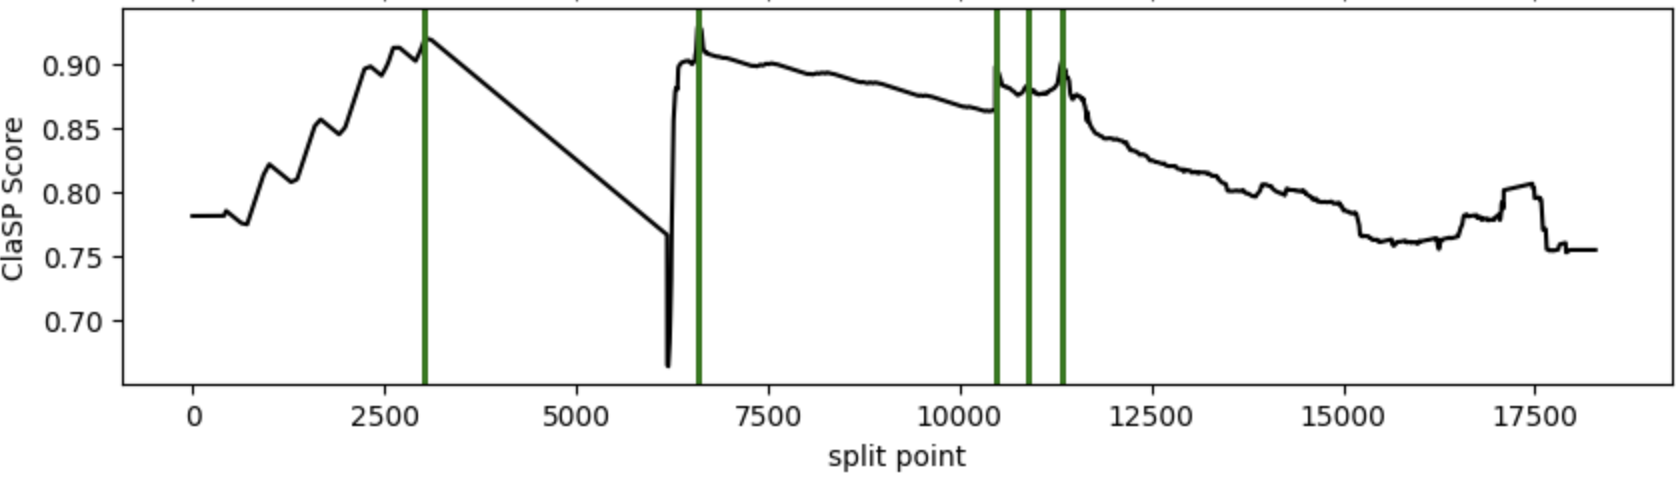
\includegraphics[width=0.45\textwidth]{img/ClaspProfile.png}
  \caption{Example of ClaSP profile. Some local maxima are selected with the Wilcoxon test to be potential changepoints of the studied time series. The red vertical lines identify the peaks considered as potential changepoints of the considered time series.}
  \label{fig:ClaSProfile}
\end{figure}

To identify potential change points, the ClaSP method looks for local maxima in the classification score profile. By locating these local maxima in the classification score profile, ClaSP highlights regions with significant dissimilarity, thus suggesting candidate positions for segmentation. 

To this point, ClaSP only detects one CP when taking the global maximum of the score profile. Achieving complete segmentation is done with a recursive algortihm which computes the score profile for the left and right segments, where each local maximum is validated as a true CP only if it statistically significant enough, namely if it passes the non-parametric Wilcoxon rank-sum test. We adapt the segmentation algorithm presented in \cite{clasp} to segment mutltivariate TS, as we expect that a complex task can generally not be fully understood when studying only one feature (position, orientation, sensor value), as relevant as it may be. Our method uses the classes available in the ClaSP code available here (lien github bas de page), but combines the profile computed for different features into one profile that contains underlying information about multiple features. As described in \ref{method_segmentation}, the combination methods explored are averaging the profiles, multiplying all the profiles and also repeating these simple methods but weighting each term by its correlation score as explained in \ref{feature_selection}. The pseudo-code of the algorithm is provided Algorithm \ref{alg:CPD}.


\begin{algorithm}
 \caption{Multivariate changepoint detection}
\begin{algorithmic}[1]
    \STATE \textbf{Procedure} check\_valid\_cp($profile$, $pq$)
    \STATE $(\text{cp\_index}, \text{cp\_val}) \leftarrow (\text{argmax(profile)}, \text{max(profile)})$
    \IF {\text{Wilcoxon\_test}(\text{cpt\_val}) passed}
        \STATE $pq$.insert(\text{cpt\_val}, (\text{cpt\_idx}, $T$))
    \ENDIF
    \STATE \textbf{end procedure}
    \STATE
    \STATE \textbf{Procedure} segmentation($T$, $combine\_method$, $min\_segmentSize$)
    \STATE cpts $\leftarrow$ initialize list
    \STATE $pq$ $\leftarrow$ initialize max priority queue
    \STATE profile $\leftarrow$ combine\_method(list\_TS, combine\_method)
    \WHILE{!$pq$.empty()}
        \STATE $(\text{cp\_index}, \text{list\_TS}) \leftarrow pq$.get\_maxPriorityValue()
        \STATE list\_T\_left, list\_T\_right $\leftarrow$ slice\_TS(list\_TS, cp\_index)
        \IF{length(list\_T\_right) $>$ min\_segmentSize}
            \STATE right\_profile $\leftarrow$ combine\_method(list\_T\_right, combine\_method)
            \STATE check\_valid\_cp(right\_profile, pq)
        \ENDIF
        \IF{length(list\_T\_left) $>$ min\_segmentSize}
            \STATE left\_profile $\leftarrow$ combine\_method(list\_T\_left, combine\_method)
            \STATE check\_valid\_cp(left\_profile, pq)
        \ENDIF
        \STATE
    \ENDWHILE
    \STATE \textbf{return} cpts
    \STATE \textbf{end procedure}
\end{algorithmic}
 \label{alg:CPD}
\end{algorithm}


\subsection{Dynamic Movement Primitives}

The concept of Discrete DMP was first introduced by Ispjeert and al. in 2002 \cite{ijspeert_movement_2002}, and more accurately developed in 2013 \cite{ijspeert_dynamical_2013}. The discrete DMP is utilized to encode a point-to-point motion into a stable dynamical system (e.g, a damped oscillator).

 A DMP for 1-DoF trajectory $y$ of a discrete movement (point-to-point) is defined by the following set of nonlinear differential equations \cite{ijspeert_movement_2002}:
\begin{align}
\tau \dot{z} &= \alpha_z \left(\beta_z(g - y) - z\right) + f(x), \label{Eq1} \\
\tau \dot{y} &= z,  \label{Eq2} \\
\tau \dot{x} &= \alpha_x x,  \label{Eq3}
\end{align}

where $x$ is the phase variable and $z$ is an auxiliary variable. Parameters $\alpha_z$ and $\beta_z$ define the behavior of the second-order system described by Equations \eqref{Eq1} and \eqref{Eq2}. Ensuring conditions $\tau > 0$, $\alpha_z = 4\beta_z$, and $\alpha_x > 0$ leads the dynamical system  to converge towards a unique attractor point at $y=g$, $z=0$ \cite{ijspeert_dynamical_2013}. In the DMP literature, Equations \eqref{Eq1}-\eqref{Eq2} are often referred to as the transformation system, while Equation \eqref{Eq3} represents the canonical system. $f(x)$ is defined as a linear combination of $N$ nonlinear Radial Basis Functions (RBFs), which allows the robot to follow any smooth trajectory from  $y_0$ to the goal $g$.

\begin{align}
f(x) &= \sum_{i=1}^{N} P_i \Psi_i(x) x,  \label{Eq4}\\
\Psi_i(x) &= \exp \left(-h_i (x - c_i)^2\right),  \label{Eq5}
\end{align}

In Equation \eqref{Eq4},  $P_i$ represents the weight associated with the $i$-th term, $\Psi_i(x)$ is defined as the $i$-th Radial Basis Function (RBF), and $x$ is the phase variable. Each RBF, given by Equation \eqref{Eq5}, is characterized by a center $c_i$ and a bandwidth parameter $h_i$.
For a given $N$ and setting $\tau$ equal to the total duration of the desired movement, we have $c_i = \exp\left(-\frac{\alpha_x(i-1)}{N-1}\right)$ and $h = \frac{1}{N(N-1)}\sum_{i=1}^{N-1}(c_{i+1}-c_i)^2$. Each degree of freedom (DoF) requires adjusting the weights $w_i$ based on the measured data to achieve the desired behavior. The number of weights should be chosen based on the desired resolution of the trajectory. When controlling a robotic system with multiple DoFs, we represent the movement of each DoF using its own equation system (1)-(2), but with a common phase (3) to synchronize them.

For a discrete motion, given a demonstrated trajectory $y_d(t_k)$, where $t_k = 1, \ldots, T$, and its time derivatives $\dot{y}_d(t_k)$ and $\ddot{y}_d(t_k)$, it is possible to invert Equation (1) and approximate the desired shape $f_d$ as follows:

\begin{equation}
f_d(t_k) = \frac{\tau^2 \ddot{y}_d(t_k) - \alpha_z \left(\beta_z (g - y_d(t_k)) - \tau \dot{y}_d(t_k)\right)}{\alpha_z}.
\label{eq:forcing-term}
\end{equation}

Equation \eqref{eq:forcing-term} provides an approximation of the desired shape $f_d(t_k)$ based on the demonstrated trajectory and its time derivatives.

By stacking each $f_d(t_k)$ and $w_i$ into the column vectors $F = \begin{pmatrix} f_d(t_1) \\ \vdots \\ f_d(t_T) \end{pmatrix}$ and $w = \begin{pmatrix} w_1 \\ \vdots \\ w_N \end{pmatrix}$, we obtain the following linear system:

\begin{equation}
\Phi w = F, 
\end{equation}

where
\begin{equation}
\Phi = \begin{bmatrix} 
    \frac{\Psi_1(x_1)}{\sum_{i=1}^{N} \Psi_i(x_1)x_1} & \ldots & \frac{\Psi_N(x_1)}{\sum_{i=1}^{N} \Psi_i(x_1)x_1} \\
    \vdots & \ddots & \vdots\\
    \frac{\Psi_1(x_T)}{\sum_{i=1}^{N} \Psi_i(x_1)x_1} & \ldots & \frac{\Psi_N(x_T)}{\sum_{i=1}^{N} \Psi_i(x_1)x_1} \\
    \end{bmatrix}
\end{equation} \newline

The phase variable $x$ in Equation \eqref{Eq3} enables the user to slow or accelerate the motion: this is the phase-stopping mechanism \cite{ijspeert_movement_2002}:

\begin{equation}
\frac{\tau_x \dot{x}}{\alpha_x} = -1 + \alpha_y x \left| \tilde{y} - y \right|, 
\end{equation}

Additionally, one useful feature of the DMP is the possibility to adapt the trajectory online if the goal changes \cite{ijspeert_dynamical_2013}:

\begin{equation}
\tau_g \dot{g} = \alpha_g (g_0 - g). 
\end{equation}

However, the standard formulation of DMPs is not suitable for directly encoding skills with specific geometric constraints, such as orientation profiles represented by unit quaternions. For instance, direct integration of unit quaternions does not ensure the unity of the quaternion's norm. Thus, the equations of the classical discrete DMP have to be adapted in order to be generalizable to quaternions. The equations system can be found in this tutorial survey about DMP \cite{saveriano_dynamic_2021}. Even though the core ideas are the same, one difference is the introduction of the \emph{quaternion logarithm} \(\text{Log}^q (\boldsymbol{gq}^* \boldsymbol{\bar{q}})\) that has an impact when it comes to computation. This expression defines the angular velocity \(\omega\) that rotates quaternion \(q\) into \(gq\) within a unit sampling time.

The function \(\text{Log}_q(\cdot) : S^3 \rightarrow \mathbb{R}^3\) is defined as:

\[
\text{Log}_q(q) = \begin{cases}
\arccos(\nu) \frac{q}{\|q\|}, & \text{if } q \neq 0 \\
[0 \ 0 \ 0]^T, & \text{otherwise}
\end{cases}
\]

This definition maps a quaternion \(q\) from the unit sphere \(S^3\) to a vector in \(\mathbb{R}^3\) using the arccosine function and normalization. 

\section{Learning from Demonstrations} \label{LfD}

\begin{figure*}[t]
  \centering
       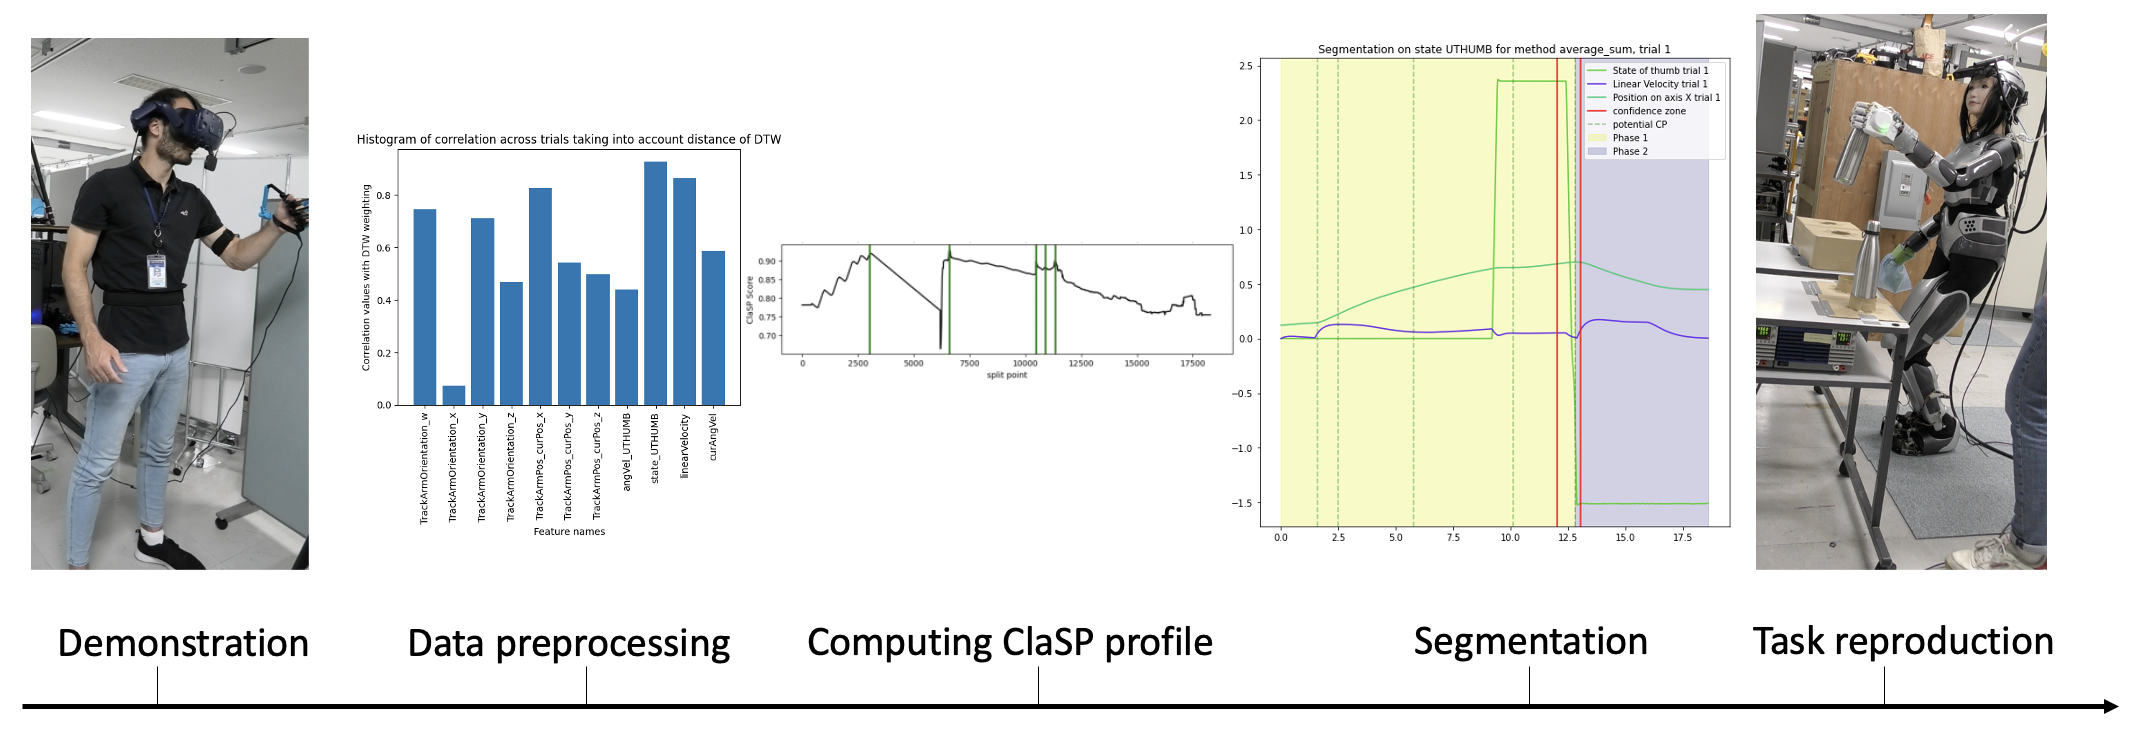
\includegraphics[width=\linewidth]{img/framework.png}
       \caption{Proposed task learning and generalization. First, we demonstrate the task with a teleoperation device (image on the left). The data is then preprocessed and features that are the most correlated (histogram on the mid-left) are selected for the segmentation with the ClaSP algorithm (image on the middle). This allows for the potential changepoints to be identified and filtered with sensor values (image on the mid-right). Finally, we can reproduce the task with Dynamic Movement Primitives on the HRP-4C robot (image on the left).\fk{texts are too small. Check all the figures.}\fk{I think it is better to use conceptual drawings instead of the real three plots.}}
     \label{fig:framework}
\end{figure*}

\subsection{Gathering demonstrations}


Building a dataset that covers a wide range of configurations is essential to reach an efficient generalization of the task, hence providing mutliple demonstrations to the robot. To do so, we demonstrated the same task in a similar environment (in the same room, with similar objects on the table, ...) but with different conditions. These include different position parameters (poses of the object, goal poses, grasping poses) as well as variate dynamic variables (speed of the movement). Having such set of demonstrations limits the \textit{covariate  shift}, that's to say the difference of distribution between the training dataset and the real-world cases. Nonetheless, we can not get rid of  this covariate shift in the extent that the action space of a given task in the real world is most often far bigger than what can represent a few demonstrations. In addition to that, our approach is to have a dataset corresponding to what might come natural to a non-professional user.

Once the demonstrations gathered, the choice of the features to study is another core step that often requires the experience of a skilled user. Whereas a great majority of LfD techniques selects manually the relevant features to study, we chose to take the measurements of all the sensors available as well as the proprioceptive information, namely 6D Cartesian position and orientation and angular and linear velocites obtained from the robot's solver. Mainly two reasons justify that:

 \begin{itemize}
     \item A non-skilled user has to be able to demonstrate a new task only by achieving it in a  natural way while wearing the teleoperation device
     \item Capitalize on our similarity with humanoid robots. Indeed, recording sensory parameters amounts to add a kind of \textit{sensory integration} to the robot. \textit{Sensory integration} was first theorized by Dr A. Jeans Ayres in 1972 in the field of neuroscience\fk{reference}. It states that when thinking about achieving some known task, our brain processes not only how to reach the goal (the different steps), but also the sensations we had when achieving this task in the past. This idea was first exploited by P. Pastor et al. in \cite{sensory_skill}. A telling example of sensory memory is that when we grab an object, the brain area corresponding to our sense of touch activates, and we expect to have some sensation when grabbing an object. In \cite{sensory_skill}, a robot arm corrects his trajectory during grabbing by adding a term that corresponds to his expected force feedback on the gripper. Thus, taking sensor into account while building the dataset can help to detect new phases of the movement \cite{sensory_seg} and correcting the movement online (after the learning phase). \newline

\end{itemize}


\subsection{Feature Selection} \label{feature_selection}

Having gathered a set of demonstrations containing numerous features, we now want to automatically extract the most relevant features to segment the task in skills reproducible with DMP.

A first step is to temporally align the signals in order to compare the features across the dataset. Indeed, our goal is to find the most correlated features. Intuitively, if one feature has the same shape in all the trials, it is likely that it will be useful for segmentation, and that it is critical to define the task. For example, in a grasping task, the opening of the gripper clearly identifies the different phases of the movement and has the same shape across all the trials. On the contrary, we expect that other parameters like the position along the z-axis have no importance in the grasping task.

To align the signals, we use Dynamical Time Warping (DTW). The main idea behind DTW is to find the optimal alignment between the two sequences by warping their time axes. This warping process allows for the matching of similar patterns, despite variations in timing and duration. It works by finding the minimum distance path through a grid or matrix that represents the pairwise distances between elements of the two sequences. \newline


We can then compute a \textit{correlation matrix} for each feature across all trials (Fig.~\ref{fig:corrMat}). The mean of the coefficients of these matrices can therefore be interpreted as the similarity across the datasets. This first result, albeit convincing, include a bias due to the temporal alignment of the signals. Indeed, it is possible to end up with a highly correlated feature when the signals are aligned, but in reality very distant. In fact, the distance computed with DTW can also be used as a tool to measure similarity. Taking again the statistical mean of the two by two distances for every feature and normalizing the values between 0 and 1, we can penalize the correlation coefficients computed afterwards. We employ the normalized DTW distances as weights for the correlation coefficients. This allows to take into account the distance between the trials, eventually leading to a more objective measure of the relevance of the features. We see in Fig.~\ref{fig:histcorr} that the most correlated features are even more detached from all the other features.  

\begin{figure}[t]
  \centering
  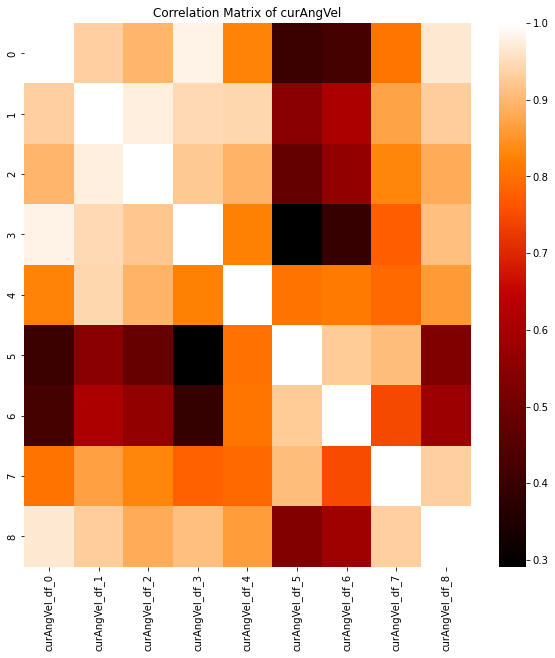
\includegraphics[width=0.45\textwidth, height = 3in]{img/resolCorrMap.png}
  \caption{Example of a correlation matrix that shows how one feature (here, the angular Velocity of the end-effector) is correlated across the 9 demonstrations.}
  \label{fig:corrMat}
\end{figure}

Finally, we select the features to pass in argument for the segmentation phase. There is a trade-off between selecting the most correlated features and discarding others - thus possibly missing important information - and choosing too much, - thus thwarting the segmentation with uncorrelated features -. In  addition to the most correlated feature $F$, we select the features that are above $CorrCoef_{F} \times T$, with $T$ a threshold that we set at $0.9$. \newline

\begin{figure}[ht]
  \centering

  \begin{minipage}[b]{0.47\linewidth}
    \centering
    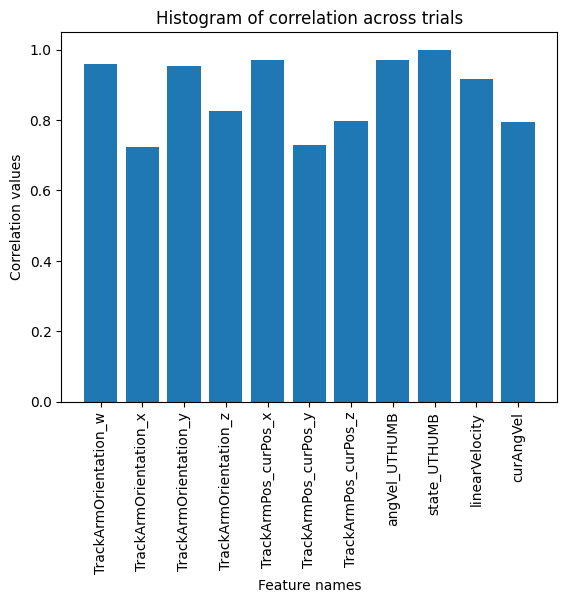
\includegraphics[width=0.9\linewidth]{img/hist_raw.png}
    \caption*{(a) Average on the correlation coefficients only}
  \end{minipage}
  \hfill
  \begin{minipage}[b]{0.47\linewidth}
    \centering
    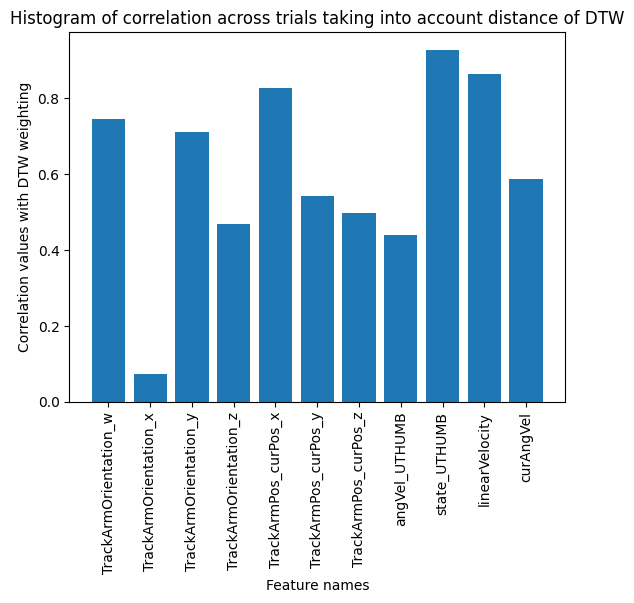
\includegraphics[width=0.9\linewidth]{img/hist_dtw.png}
    \caption*{(b) Taking into account the  distance computed with Dynamical Time Warping}
  \end{minipage}

\caption{Histogram of feature correlation across trials. The relevance of the feature is a lot clearer on the left figure that takes into account the distance computed with DTW.}
  \label{fig:histcorr}
\end{figure}

\textbf{Note:} This correlation analysis is only relevant for demonstrations that are long enough (more than a few seconds). Otherwise, the p-value of the Pearson coefficient \cite{pearson} is above 0.05 and the correlation is very likely to be irrelevant.

\subsection{Segmentation} \label{method_segmentation}

To segment demonstrations, we used the  Algorithm \ref{alg:CPD} that outputs a list  of potential CP of a multivariate time series. The default parameters of  ClaSP are used, namely the  number of estimators, the number $k$ of neighbours in the $kNN$ algorithm, the window size selection with the  SuSS algorithm. We set the parameter $min\_segmentSize = 500$, so that we only have segmented skills that have a minimum duration of one second (this paremeter excludes CPs $500$ timesteps at the right and left of the considered CP). Indeed, the timestep in mc-rtc and mc-mujoco \cite{singh2023mc} is $0.001s$, so that 1000 timesteps represent segments of 1 second. 

Then, we tried different methods to combine the profiles of the features studied. We considered averaging the profiles and multiply the profiles, but also weighted average and product. As intuitively the most correlated features have a score profile that is more relevant for the segmentation. Thus, we weight the score profiles with the correlation coefficients computed in \ref{feature_selection} before averaging or multiplying them. As we want to reduce the number of little segments, we penalize the score profile of the points next to potential breakpoints. By computing these CPs recursively, two detected CPs at step $i$ or lower are the bounds of the new time series studied at step $i+1$, we penalize the points near the edges of the profiles by applying a Kaiser filter. The output of the Kaiser filter is displayed on Fig.~\ref{fig:Kaiser}.

\begin{figure}[ht]
  \centering
  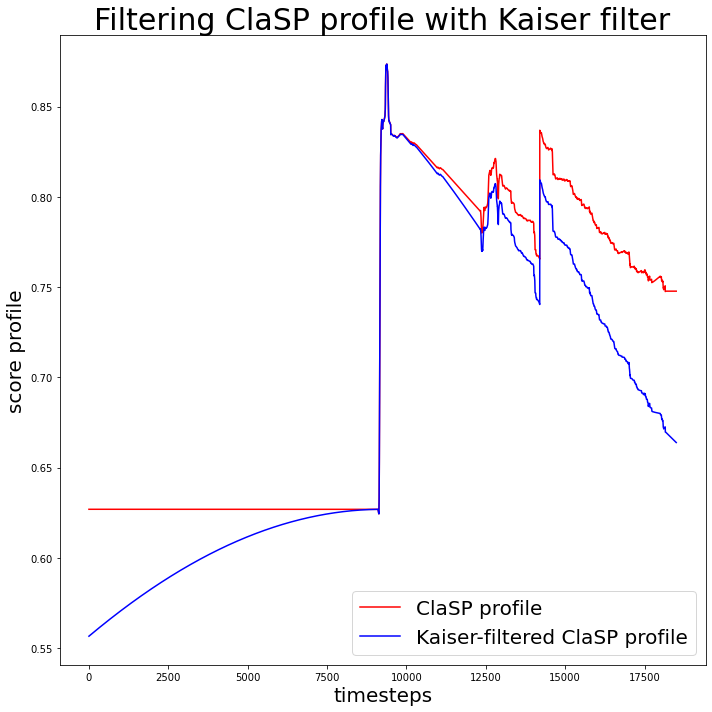
\includegraphics[width=0.45\textwidth, height=2.5
in]{img/resolKaiser.png}
  \caption{ClaSP profile after being filtered with the Kaiser filter. The value of the filtered profile fades on the edges of the profile, thus limiting the possibility to have a big sequence of short subtasks.}
  \label{fig:Kaiser}
\end{figure}

This provides us with a score profile that contains potential CPs. We then either discard or validate the changepoints thanks to sensory events. Indeed, as explored in \cite{sensory_seg}, new phases in manipulation tasks coincide  with a sensory event. We reuse this idea and compute a confidence zone around the beginning and endings of sensory events. We first clean the sensory data, that's to say remove the first difference and perform a linear regression over a sliding window to smooth the curve. Then,  we detect the sensory events  (when the data goes from a low state to a high  state and vice-versa, with a threshold set as $0.4\times max\_value$. Having detected this set of points $S$ for the time series $T$, we thus obtain the confidence zone:

\begin{equation}
        \bigcup_{s \in S} \left[ \max(0, s - \text{min\_segmentSize}),\min(s + \text{min\_segmentSize}, \text{len}(T)) \right]
\end{equation}

We finally validate the CPs computed with ClaSP if it belongs to the confidence zone. That way, we have the CPs that corresponds to the sensory events , but we do not accept CPs only if the sensors are activated.

\section{Results and discussion} \label{results}

 We first design a controller to build a dataset in  simulation on the JVRC1 virtual humanoid. To that end, we designed a finite state machine (FSM) controller with B-splines with mc-rtc \footnote{https://jrl-umi3218.github.io/mc\_rtc/index.html} and mc-mujoco \cite{singh2023mc} to simulate a one-handed grasping task of a stick in 9 different configurations as seen on Fig. \ref{fig:simSetup}. Then, we build a real-world dataset, with the JRL's teleoperation device  with the HRP-4C robot (Fig.~\ref{fig:setup}). The user has a the visual input of the humanoid's front camera, and achieves the task naturally, except that there is no force  feedback on the grippers, meaning that the demonstrator is not constrained by the physical shape of the object during the demonstrations.

 `\begin{figure}[ht]
  \centering
  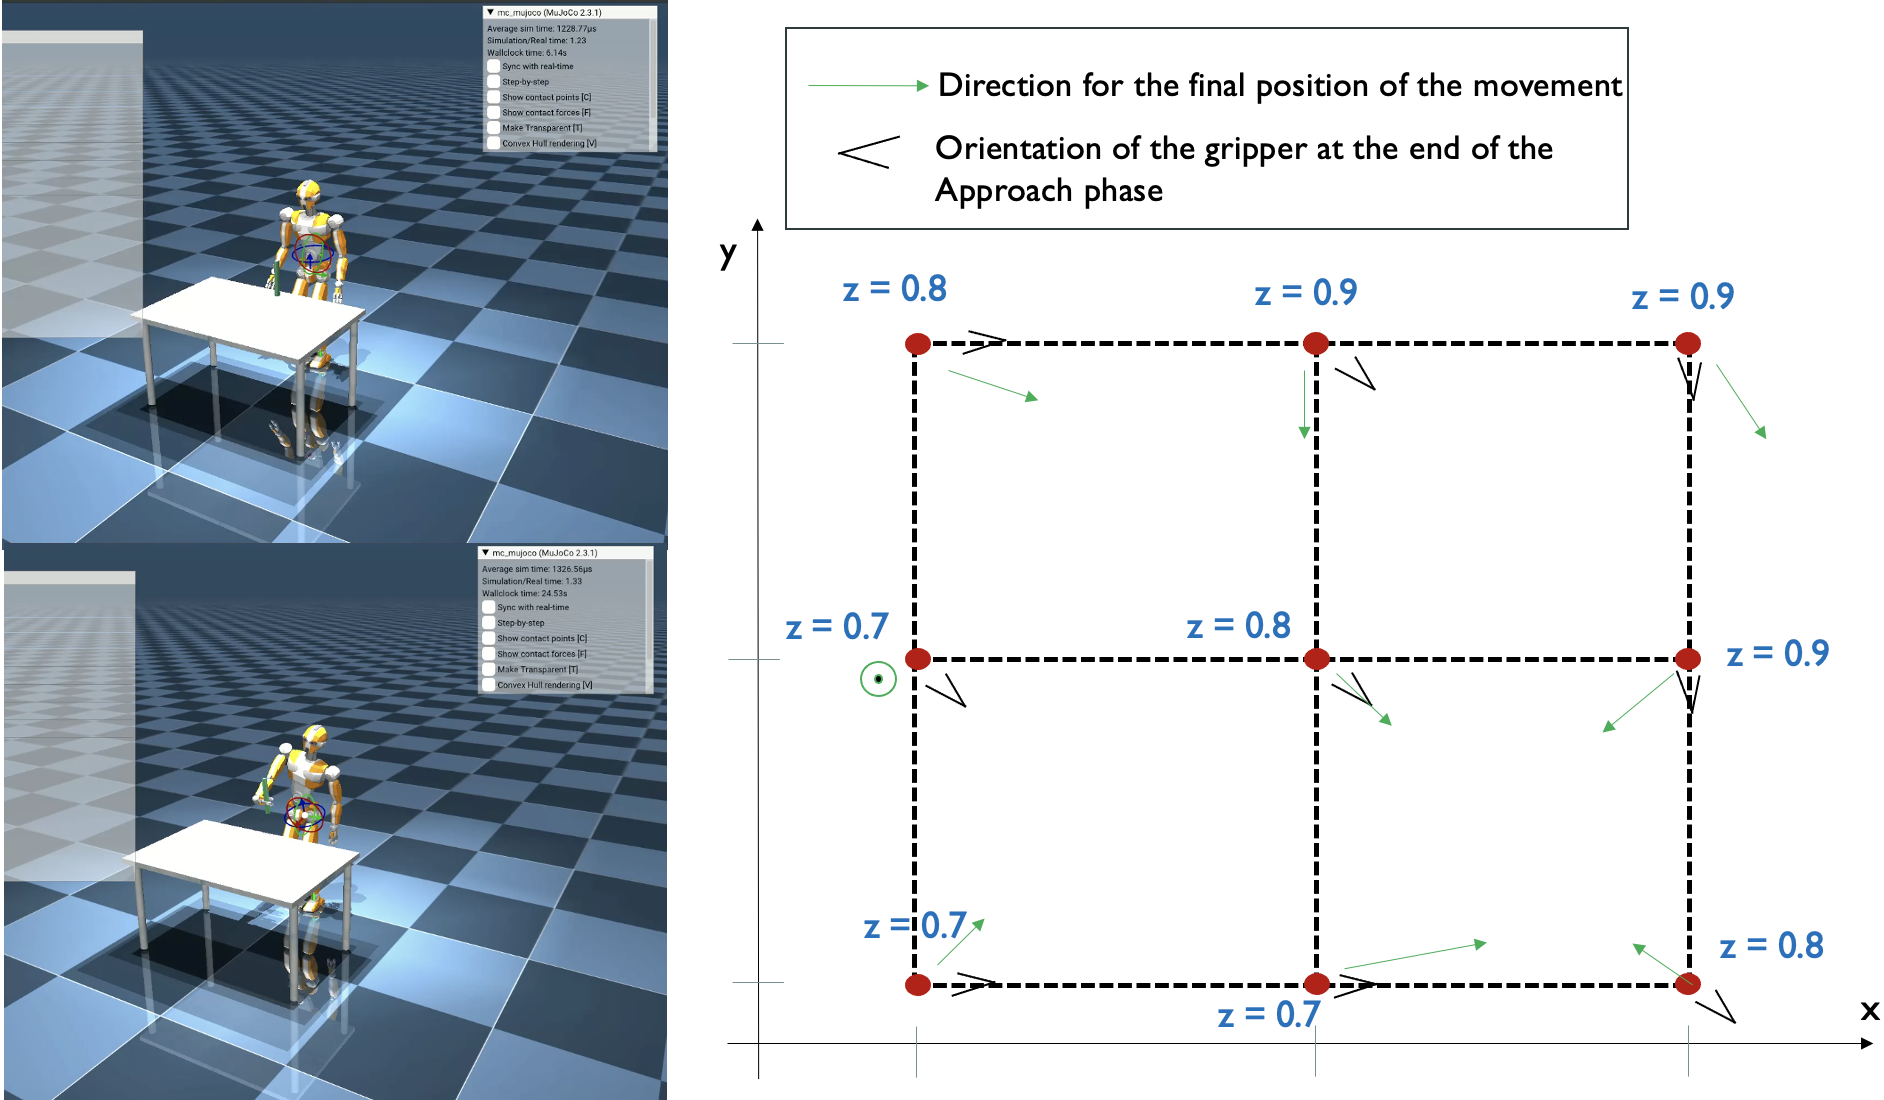
\includegraphics[width=0.45\textwidth]{img/simSetup4.png}
  \caption{Setup for the dataset built in simulation. On the left, the Mujoco interface with the JVRC-1 \cite{jvrc} at the beginning and at then end of the grasping task. On the left, the positions in which is positioned the object to grab, with the pose of the gripper before grasping the stick and the direction in which the latter is lifted.\fk{crop the screenshots to show the robot bigger.}}
  \label{fig:simSetup}
\end{figure}

 The same process is employed to build two datasets for a pushing task, where the goal is merely to push a box on a table using a hand. The video of the demonstration with teleoperation are available at \fk{incomplete}

 In both cases, mc-rtc logs all the sensor and proprioceptive values that are then used to learn and generalize the task. The task can be represented by all its normalized feature values in skill maps as in Fig. \ref{fig:skillmap}. Using this map, we have to extract appropriate features and segment it into interpretable phases. Nonetheless, the demonstrations provided with the teleoperation device are more similar to each other rather than the dataset built in simulation. That is due to the mechanical constraints of the real-robot. Those are a lot more complex in reality than in simulation.

 \begin{figure}[ht]
  \centering
  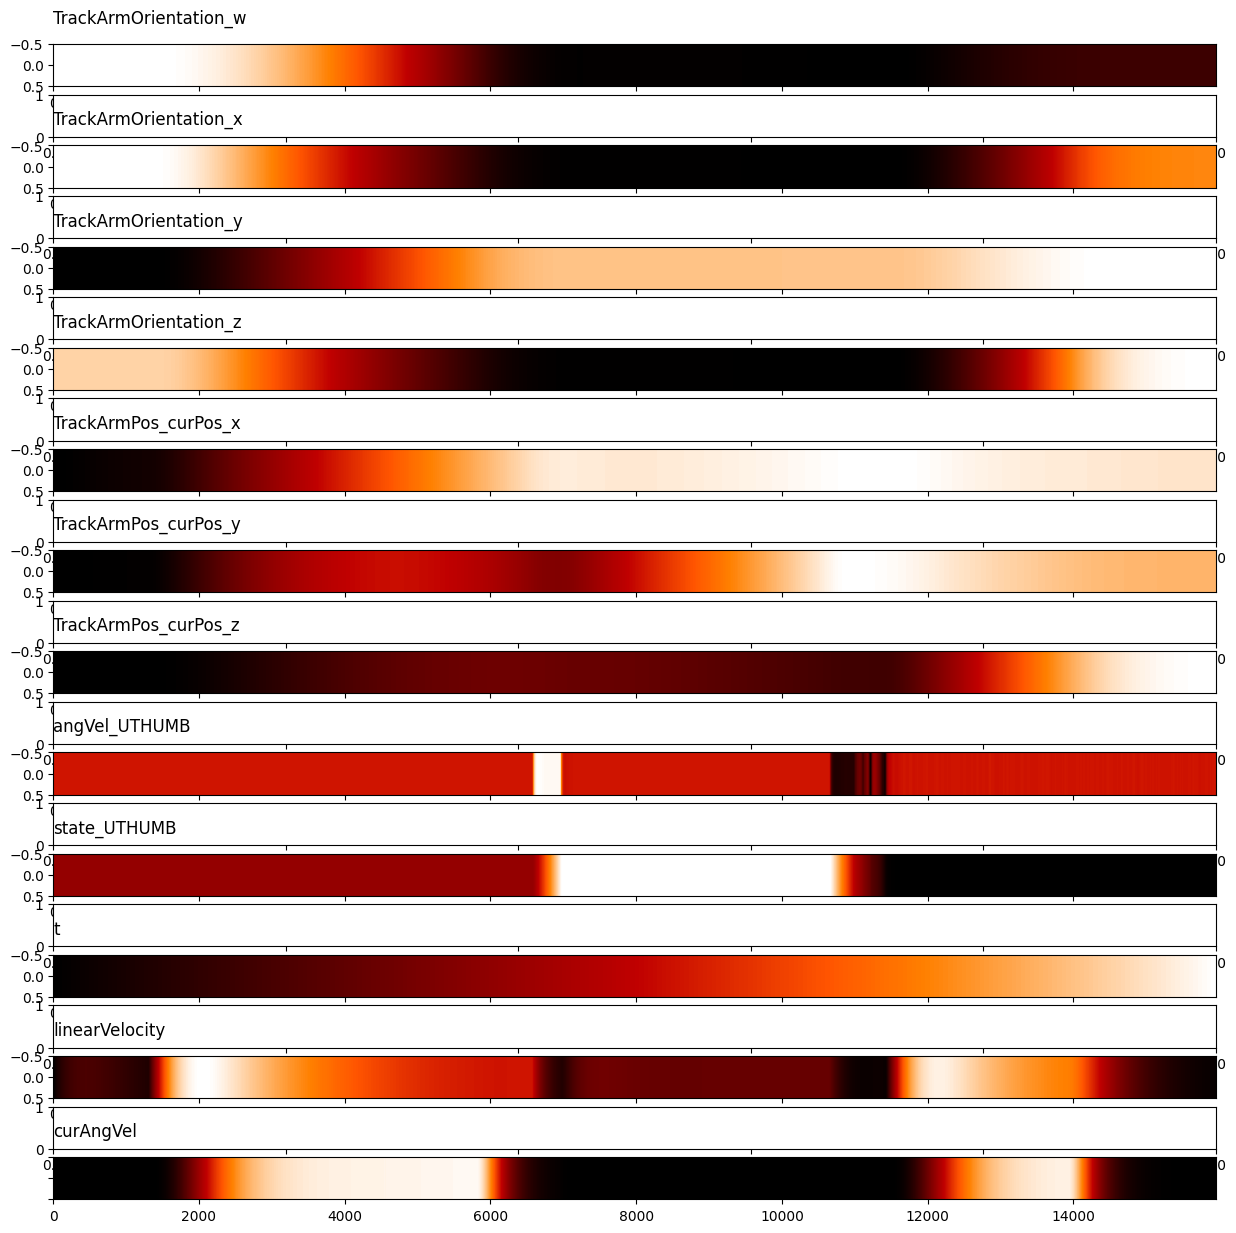
\includegraphics[width=0.45\textwidth]{img/skillMap.png}
  \caption{Representation of a task in a skill map. All the features are normalized between 0 and 1. Throughout the entire task (represented in timesteps on the abscissa), we observe the evolution of all the features studied. The higher the value of the normalized feature, the clearer on the skill map.}
  \label{fig:skillmap}
\end{figure}

To consider that a segmentation is correct, a demonstration of a grasping task must have one CP at the transition between the approach phase (when getting closer to the object) and the moving-object phase (grabbing the object and move it towards an other position). In this work, the object is not released by the robot, the task stops when the robot has lifted the object to a final position. Figure \ref{fig:coloredseg} is a correct segmentation for a grasping task.

\begin{figure}[ht]
  \centering
  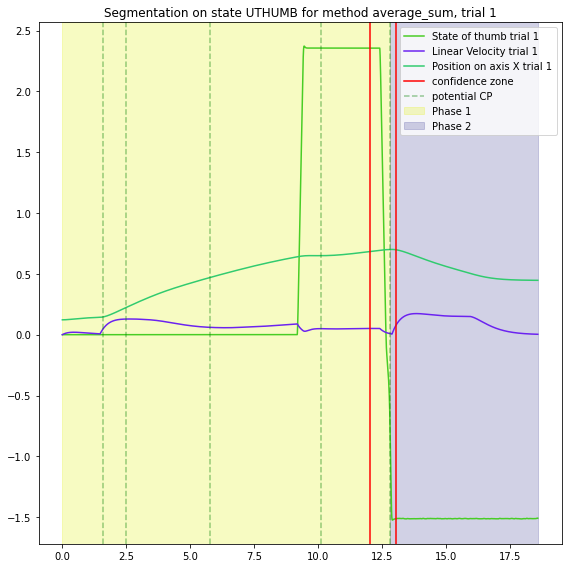
\includegraphics[width=0.5\textwidth,height=2.5in]{img/resolSeg.png}
  \caption{Correct segmentation of a grasping task. We have one CP inside the confidence zone, that is when the gripper is closing itself on the object. The different phases are coloured in beige (approach phase) and blue (move object phase).}
  \label{fig:coloredseg}
\end{figure}

As for the pushing task, two CPs are expected to be identified. We also have an approach phase when getting closer to a box to push. The pushing phase occurs when the gripper is in contact with the object. Finally, the third phase is simply returning to the initial position.

Note that we consider only correct these segmentations, but even if too much CPs are detected, the movement reproduction with DMPs will still be functional. In this case, main issues are that the segments are not interpretable by a human, and end up in task that are not learned in an optimal fashion.


Results are shown on Fig.~\ref{fig:resultsSeg} for the grasping task and the pushing task, and leads us to choose the weighted product method to compute the combined profiles. Indeed, it shows some better outcome than other methods both in simulation and on real-world data. The first striking point to this study is the lack of efficiency when going sim-to-real. While only 50\% of the demonstrations are correctly segmented in the real grasping task, the results obtained in simulation are around 80\%. This is due to noisy logs when using the teleoperation device, especially on sensory data, thus having a confidence zone that is not as accurate as that of the simulated data. We detect to much sensory events, eventually finding too much CPs (suboptimal partition of the task). Teleoperating - and more generally working with - humanoid robots that have complex hybrid behaviors ends up with having noisy data that is harder to exploit than on robots that have less DoFs (robotic arms, quadruped robots, ...).

\begin{figure}[t]
  \centering
  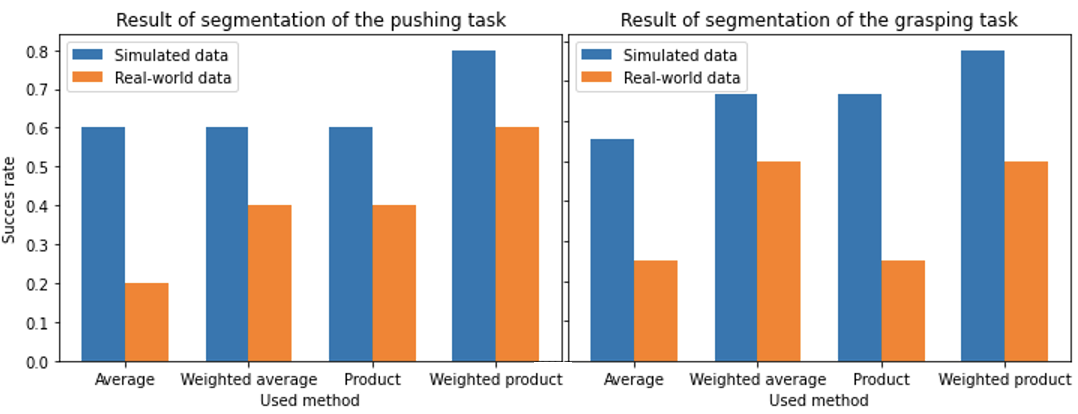
\includegraphics[width=0.5\textwidth]{img/results_segmentation.png}
  \caption{Results of the segmentation for the tasks considered. For each method studied, the results on the simulated data is in blue, and the result on the real data is in orange. The efficiency of the method on real-world data are always worse than in simulation due to the complex constraints not taken into account in simulation. While approximately 80\% of the task are successfully reproduced in simulation, the average percentage is around 50\% on the real robot.}
  \label{fig:resultsSeg}
\end{figure}

Such results can also come from the demonstrations contained in the dataset. The demonstrations provided with teleoperation are more constrained spatially and temporally. All demonstrations are more similar to each other than that of the simulation dataset. In simulation, the demonstrations covered a surface of $40 \times 40 cm$ on the table, while it is restrained to $15 \times 15 cm$ on real-world demonstrations because of the higher mechanical constraints on the HRP-4C.  We tend to have correlated features in the real world dataset that should not be correlated for the considered task, eventually leading in computing a profile that have "false" CPs that are not discarded because the sensory values (from the force or torque sensors for instance) that are too noisy. \newline

To reproduce the task, we compute DMP models for each segment of each demonstration and store them as $yaml$ files. We learn one DMP for the 6d-pose and one for the state of the gripper. Both are coordinated by the same phase variable.

When performing again this learned skill given a new goal position, we interpolate the new goal with all the precedently learned goals to find a new DMP model that fits to the task. Tasks have been reproduced using this method for the simulated grasping and pushing tasks with 100\% rate of success for the demonstrations that were correctly segmented. The execution time to reproduce the task was longer (approximately 1.5 times longer \fk{this depends on the performance of CPU. The model number needs to be mentioned. \newline
Victor/ I don't have the CPU reference of the computer I had at AIST.\newline FK:i9-10885H} due to bigger calculations at runtime to compute the next desired position with the DMP). The reproduction on the real robot is a more complex issue that is left to future work. 
\fk{no snapshots of demonstrations and reproductions? \newline
Victor: I did not have the time to perform the reproduction on the real robot. In simulation, I tested it but had not the time to record properly the task reprodution in video. I might have screenshots for the grasping task, should I add those ?\newline FK: If you have some, please add.}

\section{Conclusion and future work}\label{conclusion}

Throughout this work, we presented an end-to-end framework to learn and generalize a new task for humanoid robot by automatically segment demonstrations provided in a natural way through teleoperation into reproducible skills. In addition as being a novelty for complex humanoid robots, the proposed approach can be extended to every humanoid robot, and theoretically to every combination of end-effectors (one hand, two hands, legs). On top of that, automatically extracting the relevant features to learn the task with a correlation analysis corroborated with sensory information enables non-skilled users to learn tasks to the robots, therefore fostering humanoids integration in real-world work sites. Our approach, albeit not perfect, shows satisfactory results on simulated data (with around 80\% of success) but has to be refined to be efficient on real-world data. \newline


This work mainly paves the for two potential prolongations.
\begin{itemize}
    \item \textit{Increase the efficiency and the automation.} This would include compute 6d-pose estimation of objects based on visual input, or refine our DMP implementation to make it more efficient, add goal-switching and obstacle avoidance as stated in \cite{saveriano_dynamic_2021}. 
    
    \item  \textit{Increase the generalizability and the objectivity.} One could think about replacing the arbitrary thresholds in the feature selection or in the segmentation algorithm by statistical methods, or trying to avoid covariate shift by generating demonstrations through meta-learning \cite{yu_one-shot_2018}.

\end{itemize}
\bibliography{references.bib}
\bibliographystyle{IEEEtran}


\vspace{12pt}

\end{document}
